\section{Resultados}

\subsection{Validación de efectividad}

La primera comprobación es que los algoritmos siguen calculando $\pi$ correctamente. El protocolo de la sección 5 se aplicó antes de cronometrar nada:

\begin{center}
\small
\begin{tabular}{|l|l|r|r|r|r|c|}
\hline
\textbf{Algoritmo} & \textbf{Variante} & \textbf{Rep.} & \textbf{media $\hat\pi$} & \textbf{desv.} & \textbf{$\sigma$ teórica} & \textbf{z} \\
\hline
dartboard & serial & 20 & 3.141458 & 0.001947 & 0.001642 & 0.08 \\
dartboard & omp\_privado (T=8) & 20 & 3.141966 & 0.001574 & 0.001642 & 0.23 \\
buffon & serial & 20 & 3.141378 & 0.002152 & 0.002374 & 0.09 \\
buffon & omp\_privado (T=8) & 20 & 3.140851 & 0.002071 & 0.002374 & 0.31 \\
\hline
\end{tabular}
\caption{Test de efectividad con $N = 10^6$. Todas las medias están a menos de $0.4\sigma$ teóricas del valor real de $\pi$, y la desviación medida coincide con la teórica.}
\label{tab:validacion}
\end{center}

Dos cosas se verifican a la vez. La primera, que el estimador no está sesgado: la media de 20 corridas independientes cae praticamente sobre $\pi$. La segunda, que la \textbf{dispersión medida coincide con la predicción teórica}: para el dartboard se miden 0.001947 contra los 0.001642 previstos, y para Buffon 0.002152 contra 0.002374. Esto confirma que la fórmula de varianza de la sección 2 describe correctamente el comportamiento de los dos estimadores.

\subsection{Convergencia hacia $\pi$}

\begin{center}
\small
\begin{tabular}{|c|r|r|r|r|r|r|r|}
\hline
\multicolumn{4}{|c|}{\textbf{Dartboard}} & \multicolumn{4}{c|}{\textbf{Buffon}} \\
\textbf{N} & \textbf{$\hat\pi$} & \textbf{error} & \textbf{$\sigma$} & \textbf{N} & \textbf{$\hat\pi$} & \textbf{error} & \textbf{$\sigma$} \\
\hline
$10^3$  & 3.160000 &  0.018407 & 0.051930 & $10^3$  & 3.021148 & $-0.120445$ & 0.075057 \\
$10^4$  & 3.148400 &  0.006807 & 0.016422 & $10^4$  & 3.161056 &  0.019463 & 0.023735 \\
$10^5$  & 3.136760 & $-0.004833$ & 0.005193 & $10^5$  & 3.147970 &  0.006378 & 0.007506 \\
$10^6$  & 3.142416 &  0.000823 & 0.001642 & $10^6$  & 3.142692 &  0.001100 & 0.002374 \\
$10^7$  & 3.141216 & $-0.000377$ & 0.000519 & $10^7$  & 3.141034 & $-0.000559$ & 0.000751 \\
\hline
\end{tabular}
\caption{Convergencia de $\hat\pi$ y error absoluto frente a la desviación teórica.}
\label{tab:convergencia}
\end{center}

Todos los errores caen dentro de la banda teórica $\pm\sigma$, y la figura~\ref{fig:convergencia} muestra la convergencia y la comparación con esa banda.

\begin{figure}[ht]
\centering
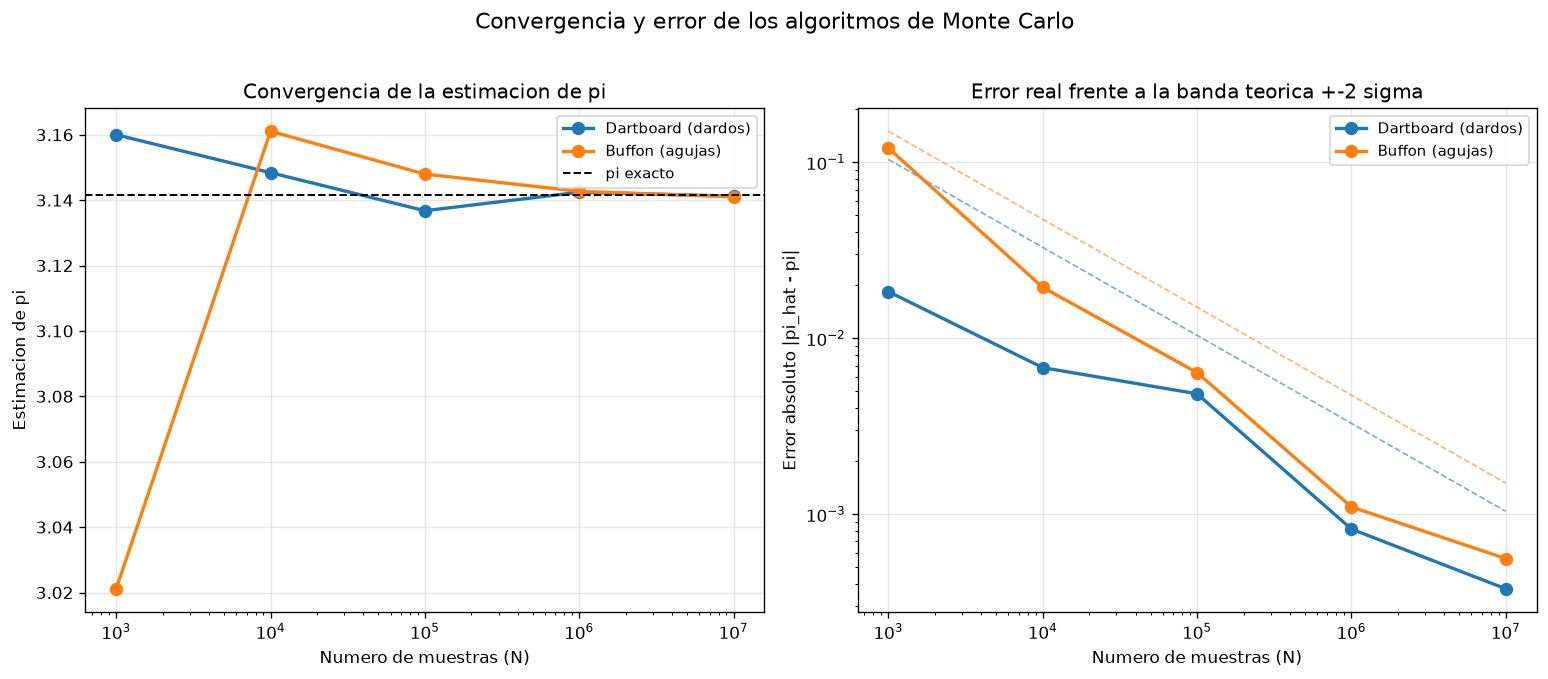
\includegraphics[width=0.98\textwidth]{figuras/convergencia_pi.png}
\caption{Convergencia de la estimación de $\pi$ (izquierda) y error absoluto frente a la banda teórica $\pm 2\sigma$ (derecha). El error real se mantiene dentro de la banda en las diez configuraciones.}
\label{fig:convergencia}
\end{figure}

La figura~\ref{fig:error} muestra el error frente a $1/\sqrt{N}$: la nube de puntos es una recta de pendiente uno, que es la ley $1/\sqrt{N}$ que predice la teoría.

\begin{figure}[ht]
\centering
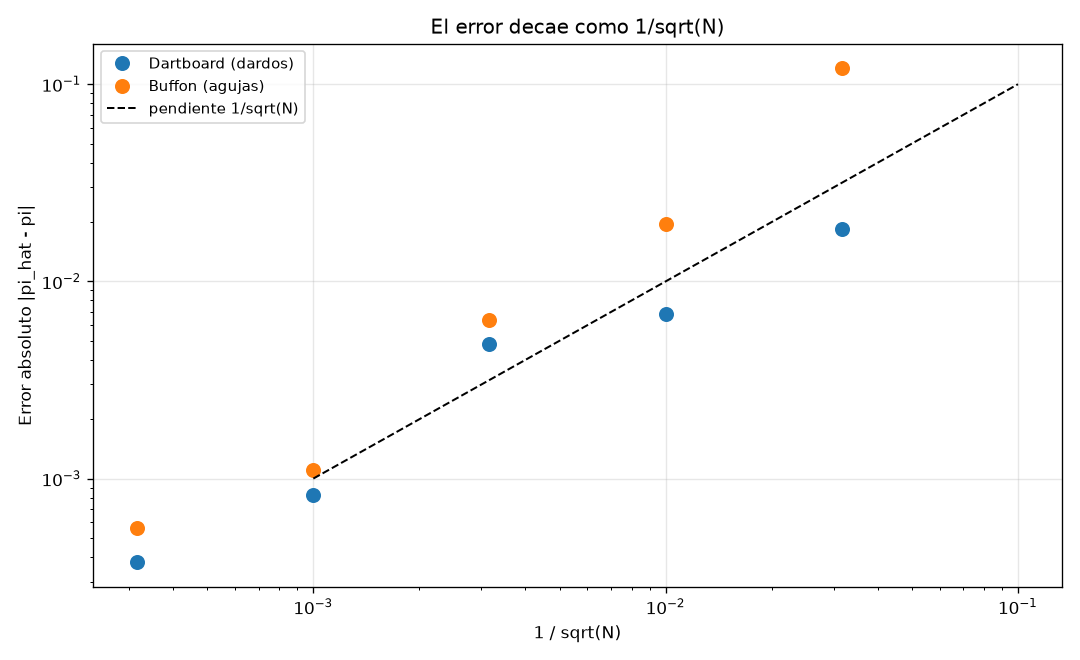
\includegraphics[width=0.8\textwidth]{figuras/error_montecarlo.png}
\caption{Error absoluto en escala logarítmica frente a $1/\sqrt{N}$. La pendiente de la recta de referencia es 1, es decir, el error decae como $1/\sqrt{N}$.}
\label{fig:error}
\end{figure}

\subsection{Perfilado de CPU: el generador de números aleatorios domina}

El perfil de GProf (sección 6.5) identifica dónde se va el tiempo:

\begin{center}
\small
\begin{tabular}{|l|r|r|r|}
\hline
\textbf{Algoritmo} & \textbf{función más costosa} & \textbf{\% del tiempo muestreado} & \textbf{instrucciones/muestra} \\
\hline
dartboard & \texttt{rng\_double} & 50.20\% & 65.0 \\
buffon & \texttt{rng\_double} & 43.64\% & 135.6 \\
\hline
\end{tabular}
\caption{Perfil de CPU con GProf ($N = 10^9$).}
\label{tab:gprof}
\end{center}

La función \texttt{rng\_double} aparece en primer lugar en ambos casos, con más de la mitad del tiempo muestreado, y el conteo de llamadas (dos por muestra, una para cada coordenada) lo confirma. La segunda diferencia está en el propio kernel: la función que contiene el bucle consume 18.62\% en Buffon frente a 8.26\% en el dartboard. Esa diferencia de unos diez puntos es precisamente el \texttt{sin}\footnote{GProf no la reporta con nombre propio porque el compilador la integra como \texttt{builtin} en la función que la contiene.} que Buffon necesita en cada muestra y el dartboard no.

\subsection{Perfilado de memoria: el conjunto de trabajo cabe en la caché}

\begin{center}
\small
\begin{tabular}{|l|r|r|r|r|r|}
\hline
\textbf{Algoritmo} & \textbf{D refs} & \textbf{D1 misses} & \textbf{D1 miss rate} & \textbf{LLd misses} & \textbf{max RSS} \\
\hline
dartboard & 250\,081\,611 & 2\,755 & \textbf{0.0\%} & 2\,063 & 2.03 MB \\
buffon & 529\,823\,078 & 2\,845 & \textbf{0.0\%} & 2\,132 & 2.32 MB \\
\hline
\end{tabular}
\caption{Perfilado de memoria con Cachegrind ($N = 10^7$).}
\label{tab:cachegrind}
\end{center}

Este es el resultado que más contraste hace con el caso de estudio anterior. Con $N = 10^7$ muestras el dartboard realiza 250 millones de referencias a datos y falla apenas 2\,755 veces en la caché L1: una tasa de fallo \textbf{de 0.0\%}, frente al 22.4\% de la multiplicación de matrices. La memoria máxima residente es de unos 2\,MB, la mayor parte del cual es el propio programa: las matrices no existen, el algoritmo es de flujo.

\begin{figure}[ht]
\centering
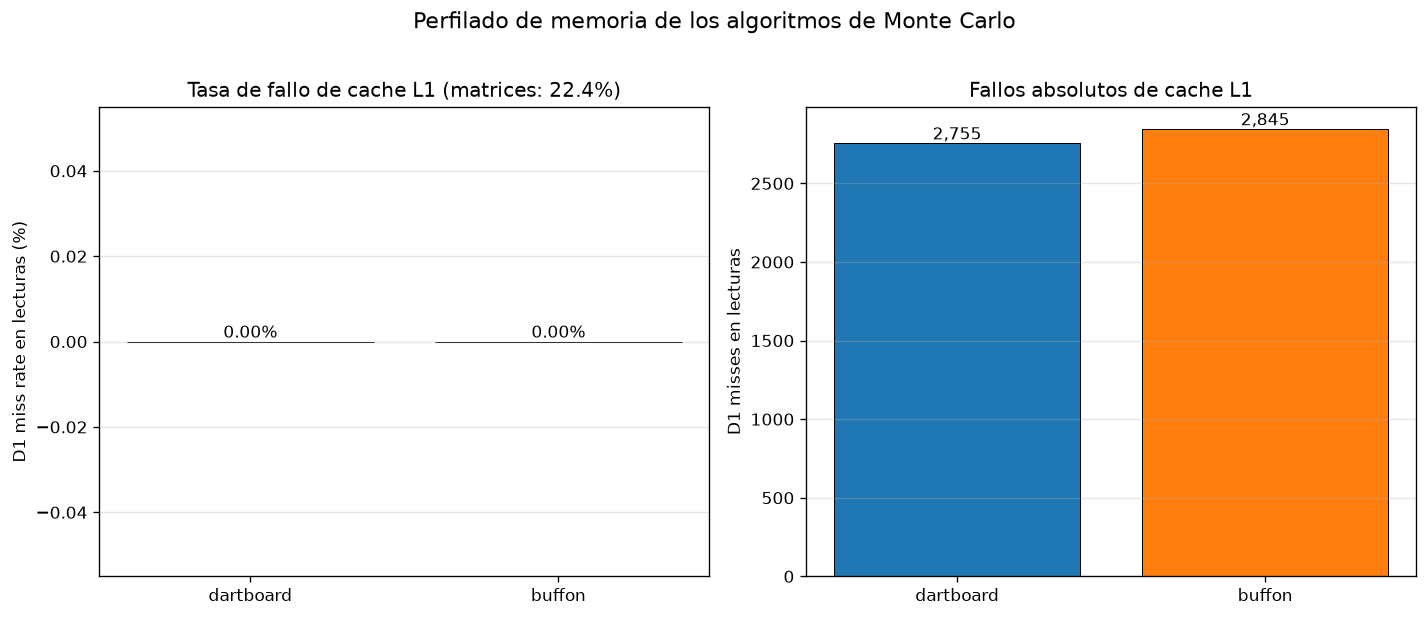
\includegraphics[width=0.85\textwidth]{figuras/cache_montecarlo.png}
\caption{Tasa de fallo de caché L1 comparada con la del kernel de multiplicación de matrices del caso de estudio 2. La diferencia explica el cambio en el comportamiento del paralelismo.}
\label{fig:cache-montecarlo}
\end{figure}

\subsection{Desempeño: escalamiento de las cuatro variantes}

La tabla~\ref{tab:speedup} muestra el speedup de cada variante frente a la versión serial, con $N = 10^9$ y tomando el mínimo de 10 repeticiones.

\begin{table}[ht]
\centering
\small
\begin{tabular}{|l|c|r|r|r|r|}
\hline
\textbf{Variante} & \textbf{T} & \textbf{dartboard} & \textbf{buffon} & \textbf{dartboard (s)} & \textbf{buffon (s)} \\
\hline
serial & 1 & 1.00$\times$ & 1.00$\times$ & 2.953 & 16.305 \\
\hline
\multirow{4}{*}{omp\_reduccion}
 & 2 & 1.40$\times$ & 1.61$\times$ & 2.110 & 10.146 \\
 & 4 & 2.02$\times$ & 2.56$\times$ & 1.465 & 6.361 \\
 & 8 & 2.67$\times$ & 3.47$\times$ & 1.108 & 4.699 \\
 & 16 & \textbf{2.75$\times$} & \textbf{3.85$\times$} & 1.075 & 4.238 \\
\hline
\multirow{4}{*}{omp\_privado}
 & 2 & 1.39$\times$ & 1.59$\times$ & 2.122 & 10.270 \\
 & 4 & 1.96$\times$ & 2.46$\times$ & 1.503 & 6.630 \\
 & 8 & 2.62$\times$ & 3.30$\times$ & 1.127 & 4.946 \\
 & 16 & 2.73$\times$ & \textbf{3.86$\times$} & 1.082 & 4.225 \\
\hline
\multirow{4}{*}{omp\_alias}
 & 2 & 0.58$\times$ & 0.75$\times$ & 5.105 & 21.846 \\
 & 4 & 0.63$\times$ & 0.67$\times$ & 4.684 & 24.221 \\
 & 8 & 0.66$\times$ & 0.84$\times$ & 4.443 & 19.306 \\
 & 16 & \textbf{0.73$\times$} & \textbf{1.45$\times$} & 4.033 & 11.223 \\
\hline
\end{tabular}
\caption{Speedup frente a la versión serial con $N = 10^9$ (mínimo de 10 repeticiones). Los tiempos en las dos últimas columnas son absolutos, en segundos.}
\label{tab:speedup}
\end{table}

\begin{figure}[ht]
\centering
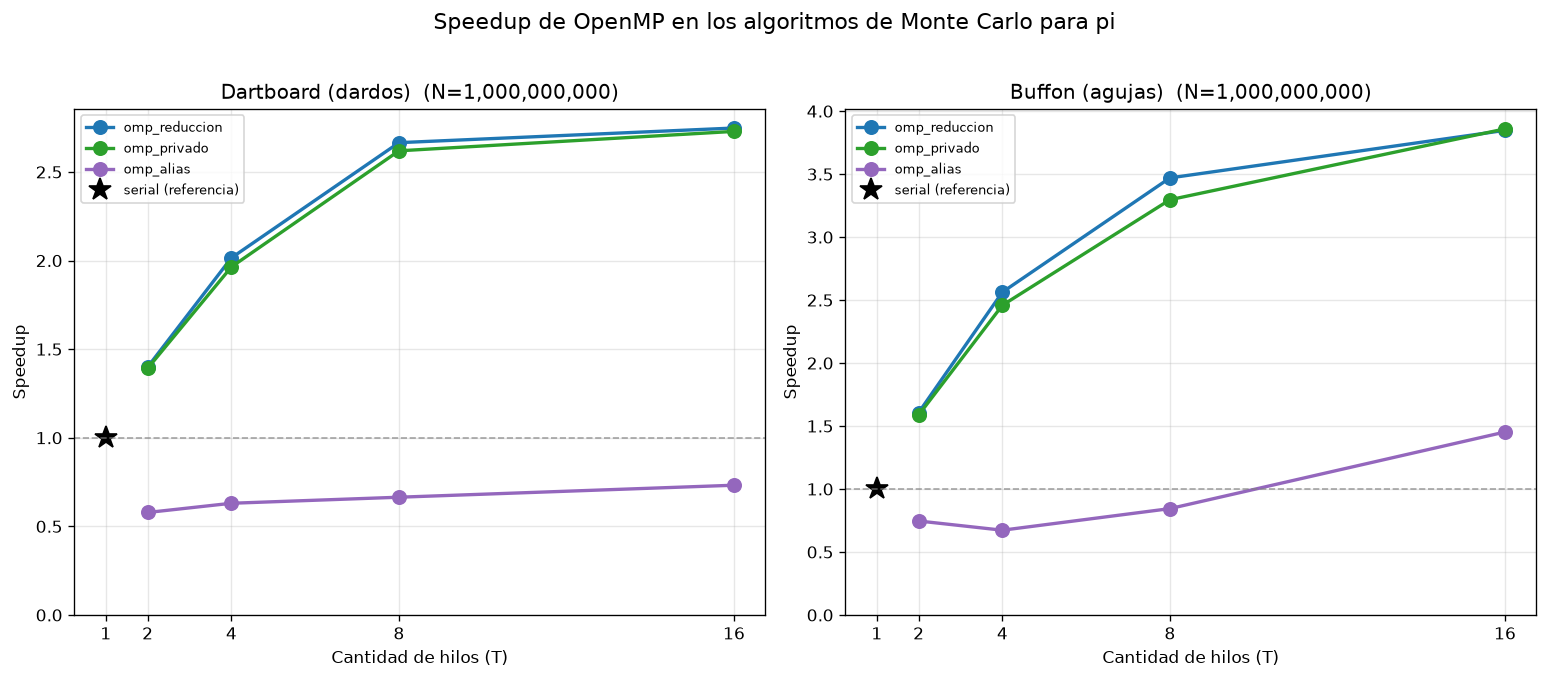
\includegraphics[width=0.98\textwidth]{figuras/speedup_montecarlo.png}
\caption{Speedup frente al número de hilos. Se observa que la variante con el estado del generador en puntero compartido (\texttt{omp\_alias}) no escala: es más lenta que la versión serial.}
\label{fig:speedup}
\end{figure}

\begin{figure}[ht]
\centering
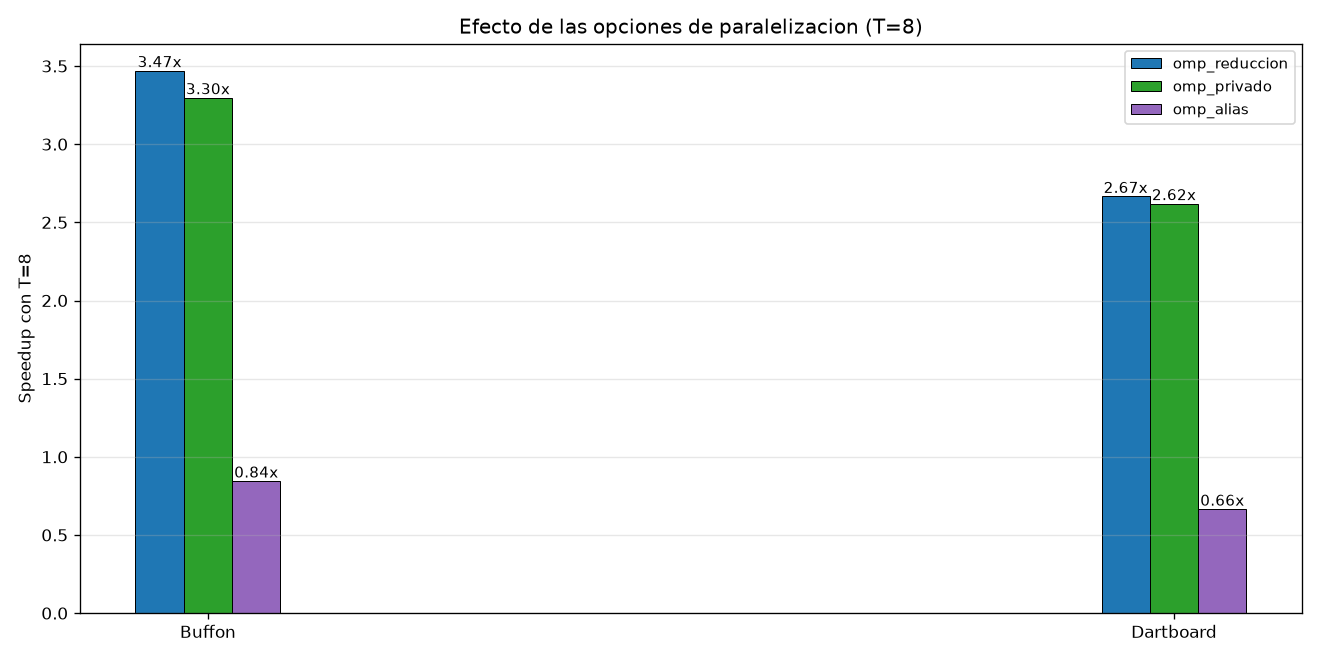
\includegraphics[width=0.85\textwidth]{figuras/escalamiento_algoritmos.png}
\caption{Efecto de cada opción de paralelización con $T = 8$. \texttt{omp\_alias} no solo escala peor, sino que empeora el tiempo respecto de la versión serial.}
\label{fig:variantes}
\end{figure}

\subsection{Costo por muestra}

\begin{figure}[ht]
\centering
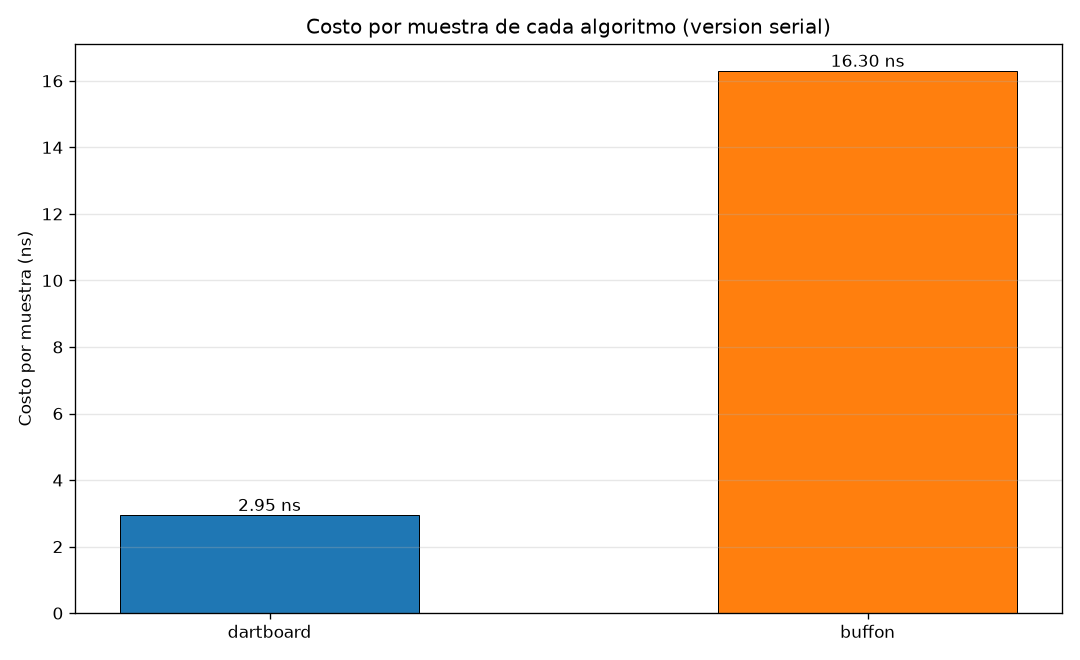
\includegraphics[width=0.75\textwidth]{figuras/costo_por_muestra.png}
\caption{Costo por muestra de cada algoritmo en la versión serial.}
\label{fig:costo}
\end{figure}

Con $N = 10^9$, el dartboard tarda 2.953\,s (2.95\,ns por muestra) y Buffon 16.305\,s (16.30\,ns por muestra). Buffon es \textbf{5.5 veces más caro por muestra}.

\subsection{Benchmark entre las dos máquinas}

\textit{[Pendiente de completar con la segunda máquina. La tabla y la gráfica quedan listas para ser rellenadas con los resultados del segundo equipo.]}

La tabla~\ref{tab:benchmark-maquinas} y la figura~\ref{fig:benchmark-maquinas} se llenan con la salida de \texttt{experiments/bench\_montecarlo.sh} ejecutado en cada equipo.

\begin{table}[ht]
\centering
\small
\begin{tabular}{|l|l|r|r|r|r|r|}
\hline
\textbf{Algoritmo} & \textbf{Máquina} & \textbf{N} & \textbf{T\_opt} & \textbf{tiempo (s)} & \textbf{ns/muestra} & \textbf{speedup} \\
\hline
dartboard & A & $10^9$ & \textit{(completar)} & & & \\
dartboard & B & $10^9$ & \textit{(completar)} & & & \\
buffon & A & $10^9$ & \textit{(completar)} & & & \\
buffon & B & $10^9$ & \textit{(completar)} & & & \\
\hline
\end{tabular}
\caption{Benchmark entre las dos máquinas. La comparación se hace con el mínimo de las repeticiones, igual que en el barrido de desempeño.}
\label{tab:benchmark-maquinas}
\end{table}

\begin{figure}[ht]
\centering
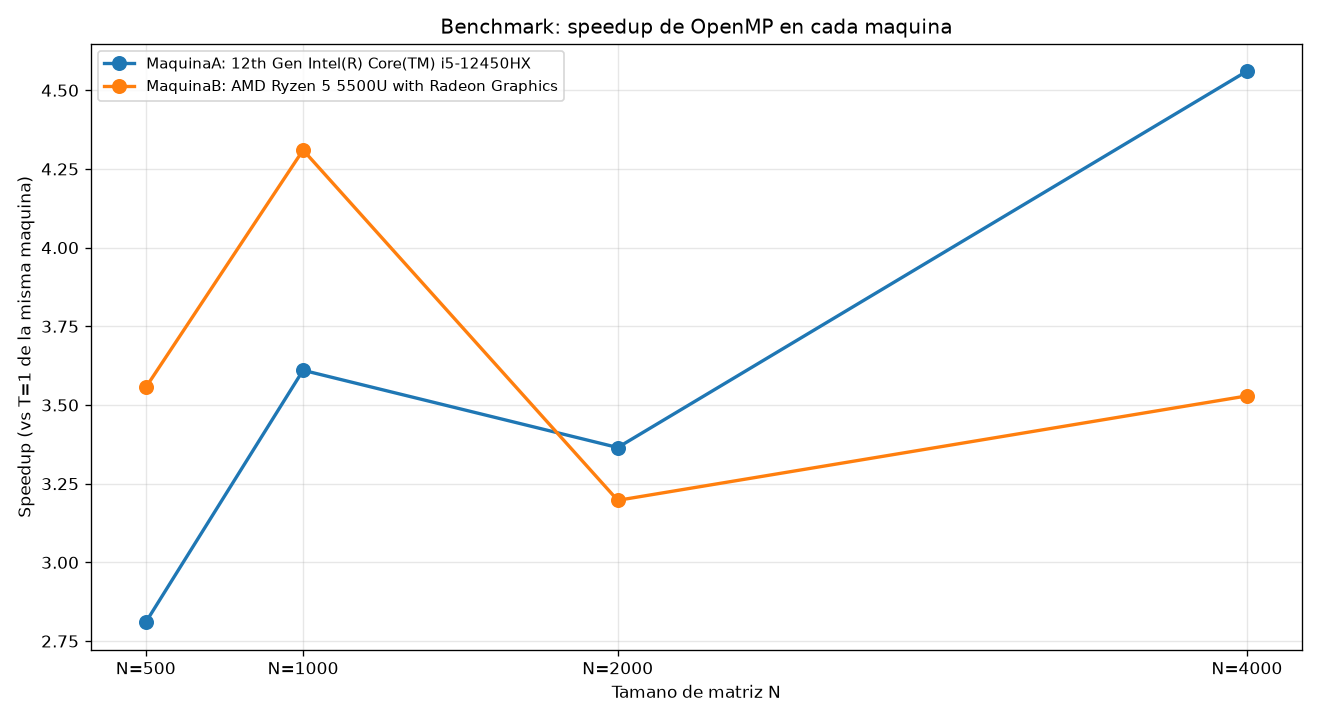
\includegraphics[width=0.95\textwidth]{figuras/benchmark_maquinas.png}
\caption{Tiempo mínimo de cada máquina para cada algoritmo y tamaño de muestra.}
\label{fig:benchmark-maquinas}
\end{figure}
